%----------------------------------------------------------------------------------------
%	DOCUMENT CONFIGURATIONS
%----------------------------------------------------------------------------------------
\documentclass[a4paper,11pt]{LaborBericht}

% ----------------------------------------------------------------------------------------
%	DOCUMENT METADATA AND VARIABLES                                                                    
% ----------------------------------------------------------------------------------------
\title{Versuch 03 - Temperaturmess- \texorpdfstring{\\}{ } technik und Wäremeableitung}
\author{Rishabh Venugopal \\ Benedikt Blattmann}
\date{\today}
\matrikelnummer{96535 (Rishabh), 96003 (Benedikt)}
\betreuer{Prof. Dr. rer. nat. Klaus Wolfrum}
% Optional - only if you need to override defaults
%\facultyname{Elektro- und Informationstechnik}
%\studiengang{Elektro- und Informationstechnik (Bachelor)}
%\titlePageGenderning{false} % Default is false, so it will be Betreuer instead of Betreuer*in. Change to true to enable genderning; ONLY ON TITLE PAGE
\berichttyp{Laborbericht Messtechnik}

% Syntax: \DeclareCaptionType{<Umgebung>}[<Bezeichnung im Abbildungsverzeichnis>][<Bezeichnung in der Überschrift>]
\DeclareCaptionType{Schaltung}[Schaltung][Schaltung]

% ----------------------------------------------------------------------------------------
% 	Begin of Document                                                                    
% ----------------------------------------------------------------------------------------
\begin{document}


%%| TABLE OF CONTENTS |%%
\maketitle
\tableofcontents
\newpage

%%| TABLE OF CONTENTS |%%
\section{Einleitung}
Temperaturmessungen spielen eine entscheidende Rolle in verschiedenen wissenschaftlichen und technischen Anwendungen. Die präzise Erfassung von Temperaturdaten ermöglicht es, physikalische Prozesse zu verstehen, Kontrollsysteme zu optimieren und Materialeigenschaften zu charakterisieren. In diesem Versuch werden die Grundlagen der Temperaturmessung sowie die Wirkprinzipien verschiedener Temperatursensoren untersucht, um ein tieferes Verständnis für diese Schlüsselkomponenten der Messtechnik zu erlangen.

\section{Vorbereitung}
\subsection{Aufgabe 1 - Temperaturabhängige Widerstände}
Um eine Temperatur in eine Elektrische Größe umzuwandeln, können temperaturabhängige Widerstände, auch Thermistor genannt, verwendet werden.
Das sind Widerstände, deren Widerstandswert sich mit der Temperatur ändert. In Schaltung \ref{fig:vorbereitung_1} ist eine Messschaltung dargestellt, mit dem man eine Messung des Widerstandes $R_T$ durchführen kann.
Hierbei wird dazu ein Spannungsteiler verwendet, der aus einem festen Widerstand $R_0$ und dem temperaturabhängigen Widerstand $R_T$ besteht.

\begin{Schaltung}[H]
    \centering
    \begin{circuitikz}[european]
        % Coordinates: Starting from (0, 3) for the top of R0

        % Top Input Terminal (extended to the left)
        \draw (-2,3) to[short, o-] (0,3);

        % Resistor R0
        \draw (0,3) to[R, -, name=R0, label=$R_0$] (0,1.5) coordinate (mid);
        %\node[right=2pt] at (0,2.25) {$R_0$}; % R0 label placement

        % Resistor RT (Variable Resistor)
        \draw (mid) to[thermistor, -, name=RT, label=$R_T$, invert] (0,0);

        % Bottom Input Terminal (extended to the left)
        \draw (-2,0) to[short, o-] (0,0);

        % Output Terminals
        % Mid Connection Point
        \node[black, fill=black, inner sep=1.5pt, circle] at (mid) {};
        \draw (mid) to[short, -o] (2,1.5); % Top output terminal

        % Bottom Connection Point
        \node[black, fill=black, inner sep=1.5pt, circle] at (0,0) {};
        \draw (0,0) to[short, -o] (2,0);   % Bottom output terminal

        % U_0 Voltage Arrow (Input - specifically placed to the left)
        \draw[->] (-1.5,2.5) -- (-1.5,0.5) node[pos=0.5, left] {$U_0$};

        % U_T Voltage Arrow (Output - specifically placed to the right, pointing down)
        \draw[->] (2.5,1.25) -- (2.5,0.25) node[pos=0.5, right] {$U_T$};

    \end{circuitikz}
    \caption{Messschaltung für temperaturabhängigen Widerstand $R_T$}
    \label{fig:vorbereitung_1}
\end{Schaltung}

Hierzu muss $R_0$ korrekt dimensioniert werden.
Es gilt den folgenden Spannungsteiler:
\begin{equation}
    U_T = U_0 \cdot \frac{R_T}{R_0 + R_T}
\end{equation}
Jetzt leiten wir $U_T$ nach $R_T$ ab, um die temperaturabhängige Spannungsänderung zu bestimmen:
\begin{equation}
    \label{eqn:temp_spannungsaenderung}
    \frac{\partial U_T}{\partial R_T} = \frac{(R_T+R_0)U_0-U_0R_T}{(R_T+R_0)^2} = U_0 \frac{R_0}{(R_T+R_0)^2}
\end{equation}
Um den Wert von $R_0$ zu ermitteln, bei dem die temperaturabhängige Spannungsänderung maximal ist, leiten wir die Gleichung \ref{eqn:temp_spannungsaenderung} nach $R_0$ ab und setzen diese gleich Null:
\begin{equation}
    \frac{\partial}{\partial R_0}\left( U_0 \frac{R_0}{(R_T+R_0)^2} \right) = U_0 \frac{R_T-R_0}{(R_T+R_0)^3}
\end{equation}
\begin{align}
    \Rightarrow U_0 \frac{R_T-R_0}{(R_T+R_0)^3} & = 0           \\
    R_T - R_0                                   & = 0 \nonumber \\
    \boxed{R_0 = R_T} \nonumber
\end{align}

Daraus folgt, dass die maximale temperaturabhängige Spannungsänderung sich bei einem Widerstandswert von $R_0 = R_T$ ergibt.

\subsection{Aufgabe 2 - PTC, NTC}
\subsubsection{pt100 Widerstand}
Der Pt100 ist ein Platin-Widerstand, welches bei seiner Bezugstemperatur (im Labor \SI{0}{\degreeCelsius}) einen Widerstand von \SI{100}{\ohm} aufweist.
Um nun den Widerstand bei einer Temperaturänderung von 1K zu bestimmen, verwenden wir die Formel eines PTC-Widerstands.
\begin{equation}
    R_{\vartheta} = R_0 \left[
        1
        + \num{3.90802e-3} \, \frac{\vartheta - \vartheta_0}{\mathrm{K}}
        - \num{5.80195e-7} \, \frac{(\vartheta - \vartheta_0)^2}{\mathrm{K^2}}
        \right]
\end{equation}

Bei PTC-Widerständen kann man in dem Temperaturbereich von \SI{0}{\degreeCelsius} bis \SI{850}{\degreeCelsius} die Kennlinie linearisieren.
\begin{figure}[H]
    
\includegraphics[width=\linewidth]{vorbereitung_kennlinie_pt100.png}
\end{figure}
Unter dieser Linearisierung ergibt sich eine Widerstandsänderung pro Kelvin von $\SI{0.375}{\frac{\ohm}{\kelvin}}$. \\
Daraus folgt: \\
$R_{25} = \SI{100}{\ohm}$ \\
$R_{26} = \SI{100.375}{\ohm}$ \\

Die relative Spannungsänderung $\frac{\Delta U_T}{U_0}$ ergibt sich damit zu:
\begin{align}
    \frac{\Delta U_T}{U_0} & = \frac{R_{T2}}{R_0 + R_{T2}} - \frac{R_{T1}}{R_0 + R_{T1}}          \nonumber                                            \\
                           & = \frac{\SI{100.375}{\ohm}}{\SI{100}{\ohm} + \SI{100.375}{\ohm}} - \frac{\SI{100}{\ohm}}{\SI{100}{\ohm} + \SI{100}{\ohm}} \\
                           & = \num{935.745e-6} \nonumber                                                                                              \\
                           & = \SI{0.09}{\percent}
\end{align}

\subsubsection{Thermistor Typ B57863S863}
Unser Thermistor ist ein NTC-Widerstand, dessen Widerstand mit steigender Temperatur abnimmt.
In diesem Fall ist die Materialkonstante $B = \SI{3988}{\kelvin}$ und der Nennwiderstand $R_N = \SI{10}{\kilo\ohm}$ bei einer Nenntemperatur von $\vartheta = \SI{25}{\degreeCelsius}$. \\
Allgemein gilt für NTC-Widerstände die folgende Formel:
\begin{equation}
    R_T = R_N \cdot e^{B \left( \frac{1}{T} - \frac{1}{T_N} \right)}
\end{equation}
Damit lassen sich auch die Widerstände für die Temperaturen \SI{25}{\degreeCelsius} und \SI{26}{\degreeCelsius} berechnen:
\begin{align*}
    R_{26}             & = \SI{10}{\kilo\ohm} \cdot e^{3988 \left( \frac{1}{299.15 \, \mathrm{K}} - \frac{1}{298.15 \, \mathrm{K}} \right)} = \SI{9.562}{\kilo\ohm}
    \\
    \frac{U_{26}}{U_0} & = \frac{R_{26}}{R_{26} + R_0} = \frac{\SI{9.562}{\kilo\ohm}}{\SI{9.562}{\kilo\ohm} + \SI{10}{\kilo\ohm}} = \num{0.4888} = \SI{48.88}{\percent} \\
    \\
    \frac{U_{25}}{U_0} & = \frac{R_{25}}{R_{25} + R_0} = \frac{\SI{10}{\kilo\ohm}}{\SI{10}{\kilo\ohm} + \SI{10}{\kilo\ohm}} = \num{0.5} = \SI{50}{\percent}             \\
\end{align*}
Die relative Spannungsänderung $\frac{\Delta U_T}{U_0}$ ergibt sich damit zu:
\begin{align*}
    \frac{\Delta U_T}{U_0} & = \frac{U_{26} - U_{25}}{U_0} = \num{0.4888} - \num{0.5} = -\num{11.19e-3} = -\SI{1.119}{\percent}
\end{align*}

\subsection{Aufgabe 3 - Auf- und Entladevorgang einer RC-Kombination}
Aufladevorgang:
\begin{equation}
    U_C(t) = U_0 \left( 1 - e^{-\frac{t}{RC}} \right)
\end{equation}
\\
Entladevorgang:
\begin{equation}
    U_C(t) = U_0 \cdot e^{-\frac{t}{RC}}
\end{equation}

\subsection{Aufgabe 4 - Grafische Bestimmung von der Zeitkonstante}
\label{sec:vorbereitung_aufgabe4}
Zur Bestimmung der Zeitkonstante $\tau$ aus der Kurve des Spannungsverlaufs $U(t)$ stehen mehrere grafische Methoden zur Verfügung.
Die erste Möglichkeit ist die Bestimmung des Wertes von $t$ bei dem die Kurve von $U(t)$ 63\% des Endwertes erreicht hat. \\
Die zweite Möglichkeit ist die Bestimmung des Wertes von $t$ bei dem die Tangente der Kurve an der Stelle $t=t_0$ die Asymptote schneidet. \\
Beide Möglichkeiten liefern den gleichen Wert für die Zeitkonstante $\tau$.

\subsection{Aufgabe 5 - Verlustleitung bei Wärmeabfuhr bei Halbleiterbauelementen}
Zur mathematischen Berechnung der Wärmeabfuhr bei Halbleiterbauelementen können wir das resultierende thermische Netzwerk als Analog zu einem elektrischen Netzwerk betrachten mit folgenden Äquivalenzen:
\begin{align*}
    \text{Verlustleistung } P_V                  & \quad \hat{=} \quad \text{Elektrischer Strom } I      \\
    \text{Temperaturdifferenz } \Delta \vartheta & \quad \hat{=} \quad \text{Elektrische Spannung } U    \\
    \text{Temperatur } \vartheta                 & \quad \hat{=} \quad \text{Knotenpotenzial } U         \\
    \text{Wärmewiderstand } R_{th}               & \quad \hat{=} \quad \text{Elektrischer Widerstand } R \\
    \text{Wärmekapazität } C_{th}                & \quad \hat{=} \quad \text{Elektrische Kapazität } C
\end{align*}
Daraus kann man bekannte Gesetze der Elektrotechnik auf die Wärmeabfuhr übertragen.
\begin{equation}
    \label{eqn:Ohmsches_Gesetz_Waerme}
    \Delta \vartheta = P_V \cdot R_{th} \quad\text{(Ohmsches Gesetz)}
\end{equation}
Bei der Wärmeabfuhr erfolgt von der Sperrschicht über das Gehäuse und den Kühlkörper zur Umgebung.
Die Verlustleistung fließt somit durch eine Reihenschaltung von Wärmewiderständen.
\begin{Schaltung}[H]
    \begin{circuitikz}[european]

        % Koordinaten definieren für saubereren Code
        \coordinate (Start) at (0,0);
        \coordinate (NodeC) at (4,0);
        \coordinate (NodeS) at (8,0);
        \coordinate (End) at (11,0);

        % Haupfad mit Widerständen und Strompfeil
        \draw (Start)
        to[short, i=$P_v$] (1.5,0)
        to[R, l_=$R_{\text{th,JC}}$] (NodeC)
        to[R, l_=$R_{\text{th,CS}}$] (NodeS)
        to[R, l_=$R_{\text{th,S}}$] (End);

        % Start-Klemme (kleiner Kreis)
        \node[ocirc] at (Start) {};

        % Vertikale Linien für die Temperaturen
        % Wir zeichnen Linien nach unten von den Knotenpunkten
        \draw ($(Start)+(0,-0.2)$) -- ++(0,-1.5) node[below] {$\theta_J$};
        \draw ($(NodeC)+(0,-0.2)$) -- ++(0,-1.5) node[below] {$\theta_C$};
        \draw ($(NodeS)+(0,-0.2)$) -- ++(0,-1.5) node[below] {$\theta_S$};
        \draw ($(End)+(0,-0.2)$)   -- ++(0,-1.5) node[below] {$\theta_a$};

        % Die Wand / Umgebung (Schraffur am Ende)
        % Vertikale Linie
        \draw (End) ++(0,1) -- ++(0,-2.5);

        % Schraffur-Linien (Loop für den Look)
        \foreach \y in {1, 0.6, ..., -1.4} {
                \draw (End) ++(0,\y) -- ++(0.5, 0.5);
            }
    \end{circuitikz}
    \caption{Ersatzschaltbild Thermisches Netzwerk zur Wärmeabfuhr bei Halbleiterbauelementen}
    \label{fig:thermisches_netzwerk}
\end{Schaltung}
Um die Verlustleistung $P_V$ bei einer Temperatur $\vartheta = \SI{125}{\degreeCelsius}$ zu ermitteln muss man
also nur die Formel \ref{eqn:Ohmsches_Gesetz_Waerme} nach $P_V$ umstellen und die entsprechenden Wärmewiderstände addieren.
\begin{equation}
    P_V = \frac{\Delta \vartheta}{R_{\text{th,gesamt}}}
\end{equation}
Die Wärmewiderstände setzen sich dabei wie folgt zusammen:
\begin{align*}
    R_{\text{th,gesamt}}     & = R_{\text{th,JC}} + R_{\text{th,CS}} + R_{\text{th,SA}}
    = \SI{3.13}{\kelvin\per\watt} + \SI{1}{\kelvin\per\watt} + \SI{15}{\kelvin\per\watt}    \\
                             & = \SI{19.13}{\kelvin\per\watt}                               \\
    R_{\text{th,gesamt,iso}} & = R_{\text{th,JC}} + R_{\text{th,CS,iso}} + R_{\text{th,SA}}
    = \SI{3.13}{\kelvin\per\watt} + \SI{2}{\kelvin\per\watt} + \SI{15}{\kelvin\per\watt}    \\
                             & = \SI{20.13}{\kelvin\per\watt}
\end{align*}
Ohne eine Isolierscheibe zwischen Gehäuse und Kühlkörper ergibt sich für die Verlustleistung:
\begin{equation}
    P_V = \frac{\Delta \vartheta_J}{R_{\text{th,JC}} + R_{\text{th,CS}} + R_{\text{th,SA}} }
    = \frac{\SI{125}{\kelvin} - \SI{25}{\kelvin}}{\SI{19.13}{\kelvin\per\watt}}
    = \SI{5.23}{\watt}
\end{equation}
Mit einer Isolierscheibe zwischen Gehäuse und Kühlkörper ergibt sich für die Verlustleistung:
\begin{equation}
    P_{V, \text{iso}} = \frac{\Delta \vartheta_J}{R_{\text{th,JC}} + R_{\text{th,CS,iso}} + R_{\text{th,SA}} }
    = \frac{\SI{125}{\kelvin} - \SI{25}{\kelvin}}{\SI{20.13}{\kelvin\per\watt}}
    = \SI{4.97}{\watt}
\end{equation}

\subsection{Aufgabe 6 - Wärmekapazität bei Wärmeabfuhr bei Halbleiterbauelementen}
Die überschlägige Berechnung der spezifischen Wärmekapazität $c_K$ des im Versuch verwendeten Kühlkörpers erfolgt über folgende Formel:
\begin{equation}
    c_K = m \cdot c_{Al} \cdot \Delta T
    = \SI{3.3}{\gram} \cdot \SI{0.9}{\frac{\kilo\joule}{\kilogram\kelvin}}
    = \SI{2.97}{\joule\per\kelvin}
\end{equation}

\subsection{Aufgabe 7 - Stationäre Temperatur}
Um die Zeit zu ermitteln, die der Kühlkörper benötigt, um eine stationäre Temperatur zu erreichen, modellieren wir das thermische Netzwerk als RC-Glied.
Die Zeitkonstante $\tau$ ergibt sich aus dem Produkt von Wärmewiderstand und Wärmekapazität:
\begin{align}
    \tau              & = R_{\text{th,gesamt}} \cdot C_K = \SI{19.13}{\kelvin\per\watt} \cdot \SI{2.97}{\joule\per\kelvin}     \\ & = \SI{56.8}{\second} \nonumber \\
    \tau_{\text{iso}} & = R_{\text{th,gesamt,iso}} \cdot C_K = \SI{20.13}{\kelvin\per\watt} \cdot \SI{2.97}{\joule\per\kelvin} \\ & = \SI{59.8}{\second} \nonumber
\end{align}
Die Temperatur erreicht nach $5\tau$ ca. 99\% des Endwertes, wird also praktisch stationär.
Somit ergibt sich die Zeit bis zur stationären Temperatur zu:
\begin{align}
    t_{\text{stationär}}     & = 5 \cdot \tau = 5 \cdot \SI{56.8}{\second} = \SI{284.05}{\second} = \SI{4.73}{\minute}             \\
    t_{\text{stationär,iso}} & = 5 \cdot \tau_{\text{iso}} = 5 \cdot \SI{59.8}{\second} = \SI{299.9}{\second} = \SI{4.98}{\minute}
\end{align}

\subsection{Aufgabe 8 - Berechnung von RT}
Um den Widerstand $R_T$ in Abhängigkeit von $U_{ref}$ und $R_0$ zu berechnen, wird der Spannungsteiler aus Schaltung \ref{fig:vorbereitung_1} verwendet.
\begin{alignat}{2}
    \label{eqn:a8}
    % Zeile 1: Kein Pfeil, leere erste Spalten
                    & \quad & U_{T}                                            & = U_{ref} \cdot \frac{R_T}{R_0 + R_T} \nonumber   \\
    % Zeile 2: Pfeil in Spalte 1, Gleichung in Spalte 2
    \Leftrightarrow &       & R_T                                              & = (R_T + R_0) \cdot \frac{U_T}{U_{ref}} \nonumber \\
    \Leftrightarrow &       & R_T - R_T \cdot \frac{U_T}{U_{ref}}              & = R_0 \cdot \frac{U_T}{U_{ref}} \nonumber         \\
    \Leftrightarrow &       & R_T \cdot \left( 1 - \frac{U_T}{U_{ref}} \right) & = R_0 \cdot \frac{U_T}{U_{ref}}                   \\
    \Leftrightarrow &       & R_T \cdot \frac{U_{ref} - U_T}{U_{ref}}          & = R_0 \cdot \frac{U_T}{U_{ref}} \nonumber         \\
    \Leftrightarrow &       & R_T                                              & = R_0 \cdot \frac{U_T}{U_{ref} - U_T} \nonumber
\end{alignat}

\subsection{Aufgabe 9}
Die Spannung $U_T$ wird vom SAR-ADC gemessen und als Zahlenwert $Z$ ausgegeben. Allgemein gilt für $Z$, der bei einem 12-Bit SAR-ADC mit einer Eingangsspannung $U_T$ und einer Vollausschlagspannung $U_{\text{SAR,max}} = 2U_{\text{ref}}$ und $Z_{\text{SAR,max}} = 4095 = 2^{12} - 1$:
\begin{alignat}{2}
    \label{eqn:a9}
                    & \quad & \frac{Z}{Z_{\text{SAR,max}}} & = \frac{U_T}{U_{\text{SAR,max}}}                                 \\
    \Leftrightarrow &       & Z                            & = \frac{U_T}{2U_{\text{ref}}} \cdot Z_{\text{SAR,max}} \nonumber
\end{alignat}

\subsection{Aufgabe 10}
Unter Verwendung der Ergebnisse aus Aufgabe 8 und 9 kann nun gezeigt werden, dass
$R_T$ unabhängig von $U_{\text{ref}}$ ist.
Dazu setzen wir die Gleichung \ref{eqn:a9} in die Gleichung \ref{eqn:a8} ein:
\begin{alignat}{2}
    \label{eqn:a10}
                    & \quad & R_T & = R_0 \cdot \frac{\frac{Z}{Z_{\text{SAR,max}}} \cdot 2U_{\text{ref}}}{U_{\text{ref}} - \frac{Z}{Z_{\text{SAR,max}}} \cdot 2U_{\text{ref}}} \nonumber \\
    \Leftrightarrow &       &     & = R_0 \cdot \frac{\frac{2Z}{Z_{\text{SAR,max}}} \cdot U_{\text{ref}}}{U_{\text{ref}} \left( 1 - \frac{2Z}{Z_{\text{SAR,max}}} \right)}               \\
    \Leftrightarrow &       &     & = R_0 \cdot \frac{2Z}{Z_{\text{SAR,max}} - 2Z} \nonumber
\end{alignat}

\subsection{Aufgabe 11}
Unter der Annahme, dass der SAR-ADC den Zahlenwert $Z = 1024$ ausgibt und $R_0 = \SI{10}{\kilo\ohm}$, ergibt sich für den Widerstand $R_T$:
\begin{equation}
    R_T = R_0 \cdot \frac{2Z}{Z_{\text{SAR,max}} - 2Z} = \SI{10}{\kilo\ohm} \cdot \frac{2 \cdot 1024}{4095 - 2 \cdot 1024} = \SI{10.00489}{\kilo\ohm}
\end{equation}
Um die zugehörige Temperatur zu bestimmen wird die Steinhart-Hart-Gleichung verwendet:
\begin{equation}
    \frac{1}{T} = A + B \cdot \ln(R_T) + C \cdot (\ln(R_T))^3
\end{equation}
Mit den Konstanten aus der Vorbereitung
\begin{align*}
    A & = \SI{1.12559726e-03}{\per\kelvin} \\
    B & = \SI{2.34801612e-04}{\per\kelvin} \\
    C & = \SI{8.63986114e-08}{\per\kelvin}
\end{align*}
und $R_T = \SI{10.00489}{\kilo\ohm}$ ergibt sich für die Temperatur:
\begin{align*}
    \frac{1}{T} & = \SI{1.126e-3}{\per\kelvin} + \SI{2.348e-4}{\per\kelvin} \cdot \ln\left(\frac{\SI{10004.89}{\ohm}}{\SI{1}{\ohm}}\right) \\
                & \quad + \SI{8.640e-8}{\per\kelvin} \cdot \ln^3\left(\frac{\SI{10004.89}{\ohm}}{\SI{1}{\ohm}}\right)                      \\
                & = \SI{3.3558e-3}{\per\kelvin}                                                                                            \\
\end{align*}

\begin{equation}
    \Rightarrow \boxed{T = \SI{297.989}{\kelvin} \approx \SI{25}{\degreeCelsius}}
\end{equation}



\section{Versuchsdurchführung}
\subsection{Versuchsaufbau}
\subsubsection{Hardware}
Der Versuchsaufbau besteht aus zwei Platinen:
\begin{itemize}
    \item \textbf{Transistorplatine:} Diese beinhaltet die Leistungstransistoren und die Temperatursensoren.
    \item \textbf{Controllerplatine:} Diese dient zur Messerfassung mittels eines PSoC.
\end{itemize}
\begin{figure}[H]
    \centering
    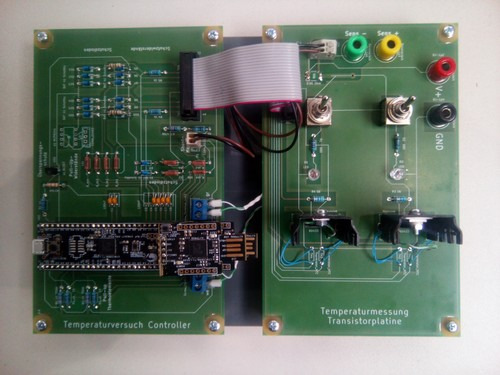
\includegraphics[width=0.7\textwidth]{images/versuchsschaltung.jpeg}
    \caption{Übersicht über die gesamte Versuchsschaltung mit Controllerplatine links
        und Transistorplatine rechts.}
    \label{fig:versuchsschaltung}
\end{figure}
Auf der Transistorplatine sind zwei Leistungstransistoren zum Ausmessen aufgebaut. Diese sind mit einem Kühlkörper verbunden, auf dem sich die Temperatursensoren befinden. Der Unterschied zwischen den beiden Transistoren besteht darin, dass einer mit einer zusätzlichen Keramikscheibe zur thermischen Isolation ausgestattet ist. Die Controllerplatine beinhaltet den PSoC-Mikrocontroller, der die Messwerte der Temperatursensoren ausliest und an den PC weiterleitet. 

Zum Aufheizen des Transistors wird ein Labornetzgerät verwendet, dessen Ausgangsstrom auf \SI{1.5}{\ampere} begrenzt ist. Um die Kollektor-Emitter-Spannung und den Strom in der Software zu überwachen, werden zwei Digitalmultimeter verwendet. Diese kommunizieren über eine serielle Schnittstelle mit dem PC.

\subsubsection{Software}
Zur Visualisierung der Messergebnisse wird eine Python-Software verwendet, welche die Daten vom PSoC-Mikrocontroller über eine serielle Schnittstelle empfängt und in Echtzeit darstellt. 
Es gibt die Möglichkeit, zwischen den beiden Transistoren zu wählen. Je nach ausgewähltem Transistor können bis zu drei verschiedene Temperatursensoren dargestellt werden. Um eine Messung zu starten, muss zunächst die Messdauer angegeben und anschließend die Verbindung zur Platine überprüft werden. 
Nach Ende der Messung werden die Daten in einer CSV-Datei und als Bild gespeichert. 

\subsection{Durchführung}
Es gibt insgesamt zwei Messdurchläufe, jeweils einen pro Transistor. Pro Transistor wird für eine Zeitdauer von $10\tau$, d.h. \SI{1200}{\second}, gemessen. Hierbei werden für jeweils \SI{600}{\second} die Aufheizphase und die Abkühlphase erfasst. Um eine korrekte Messung zu erhalten, muss eine Basislinie erfasst werden, indem der jeweilige Schalter erst ca. \SI{15}{\second} nach Start der Messung umgelegt wird.
\section{Auswertung und Analyse}
\begin{figure}[H]
    \centering
    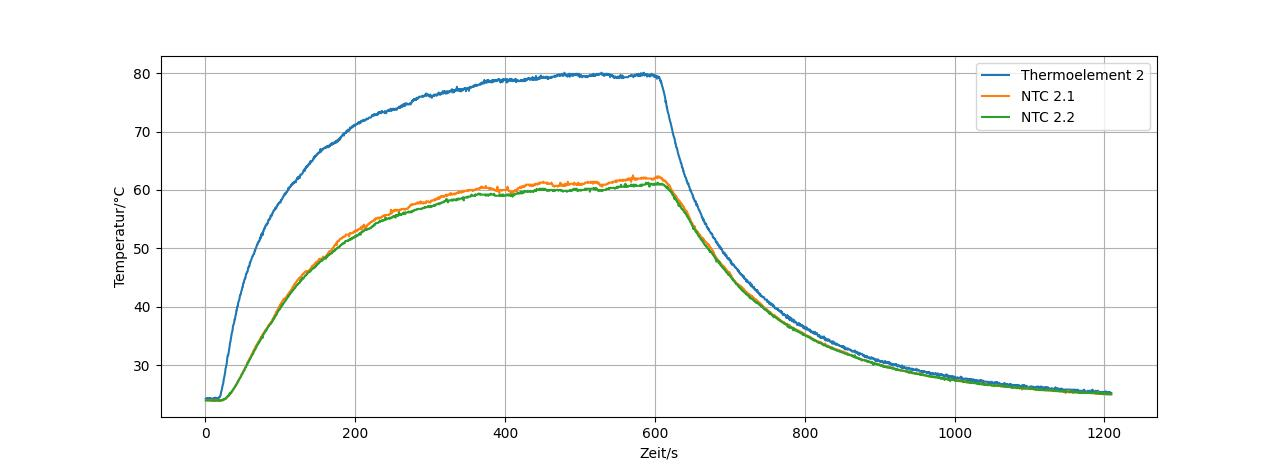
\includegraphics[width=0.9\textwidth]{data/temperatur_messung_mit_scheibe_16_00_.jpg}
    \caption{Temperaturverlauf mit Keramikscheibe}
    \label{fig:temperaturverlauf_mit_isolierung}
\end{figure}
\begin{figure}[H]
    \centering
    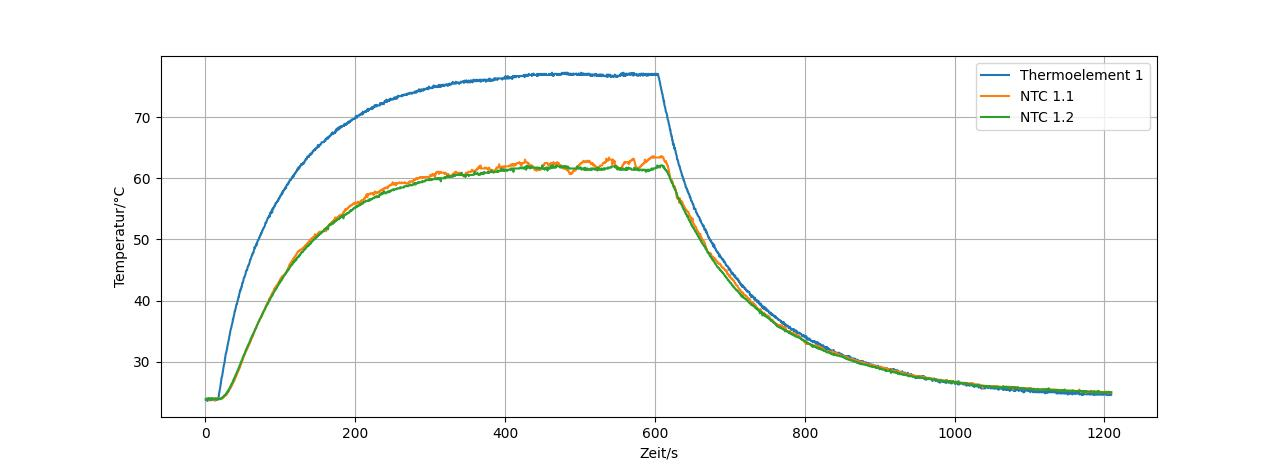
\includegraphics[width=0.9\textwidth]{data/temperatur_messung_ohne_scheibe_16_25_.jpg}
    \caption{Temperaturverlauf ohne Keramikscheibe}
    \label{fig:temperaturverlauf_ohne_isolierung}
\end{figure}

\subsection{Aufheizphase}
Die Aufheizphase erstreckt sich in einem Zeitberich von ca. \SI{15}{\second} bis \SI{610}{\second}. In diesem Zeitraum erwärmen sich die Transistoren von Raumtemperatur auf ihre Beharrungstemperatur.
Die Beharrungstemperatur geht aus aun Graphen der Messungen vor, dargestellt in Abbildung \ref{fig:temperaturverlauf_mit_isolierung} und Abbildung \ref{fig:temperaturverlauf_ohne_isolierung}.
\begin{table}[H]
    \centering
    \begin{tabular}{l|c|c}
        \toprule
        \textbf{Temperatursensor} & \textbf{Mit Isolierung}     & \textbf{Ohne Isolierung}    \\
        \midrule
        Thermoelement             & \SI{79.586}{\degreeCelsius} & \SI{76.913}{\degreeCelsius} \\
        NTC1                      & \SI{61.514}{\degreeCelsius} & \SI{62.528}{\degreeCelsius} \\
        NTC2                      & \SI{60.459}{\degreeCelsius} & \SI{61.539}{\degreeCelsius} \\
        \bottomrule
    \end{tabular}
    \caption{Beharrungstemperaturen der verschiedenen Sensoren}
    \label{tab:beharrungstemperaturen}
\end{table}
Wie in Kapitel \ref{sec:vorbereitung_aufgabe4} beschrieben, kann man nun beobachten wie lange es dauert, bis die Transistoren 63\% ihrer Beharrungstemperatur erreicht haben. Hierbei wird die Zeitkonstante $\tau$ bestimmt, indem die Kurve als PT2-System angenähert wird. Dafür wird das bereitgestellte Pythonprogramm zur Parameteridentifikation verwendet. Die Ergebnisse sind in Tabelle \ref{tab:taus} dargestellt.
\begin{table}[H]
    \centering
    \renewcommand{\arraystretch}{1.2}
    \begin{tabular}{lcccc}
        \toprule
                      & \multicolumn{2}{c}{\textbf{Mit Isolierung}} & \multicolumn{2}{c}{\textbf{Ohne Isolierung}}                                                      \\
        % \cmidrule(lr){2-3} draws a line only under columns 2 and 3 (trimmed Left and Right)
        \cmidrule(lr){2-3} \cmidrule(lr){4-5}
        Sensor        & $\tau$                                      & $T_{63\%}$                                   & $\tau$               & $T_{63\%}$                  \\
        \midrule
        Thermoelement & \SI{95.209}{\second}                        & \SI{59.105}{\degreeCelsius}                  & \SI{89.960}{\second} & \SI{57.263}{\degreeCelsius} \\
        NTC1          & \SI{112.264}{\second}                       & \SI{47.612}{\degreeCelsius}                  & \SI{95.062}{\second} & \SI{48.229}{\degreeCelsius} \\
        NTC2          & \SI{112.112}{\second}                       & \SI{46.951}{\degreeCelsius}                  & \SI{96.156}{\second} & \SI{47.610}{\degreeCelsius} \\
        \bottomrule
    \end{tabular}
    \caption{Zeitkonstanten und 63\%-Temperaturen der Aufheizphase}
    \label{tab:taus}
\end{table}
Hier kann man erkennen, dass die Zeitkonstanten bei dem Transistor mit Isolierung größer sind als bei dem Transistor ohne Isolierung. In einfachen Worten heißt es, dass der Transistor mit Isolierung sich langsamer aufheizt. Dies liegt daran, dass die Keramikscheibe die Wärmeabfuhr des Transistors erschwert, wodurch sich die Temperatur langsamer erhöht.
Das Programm nähert die Kurve als PT2-System an und gibt die Plotparameter aus, welche in Abbildung \ref{fig:plotparam_aufheiz_mit_isolierung_te} und Abbildung \ref{fig:plotparam_aufheiz_ohne_isolierung_te} dargestellt sind. Im prinzip werden die Parameter an der modellmäßg zu erwartenden Sprungantwort angepasst.
\begin{figure}[H]
    \centering
    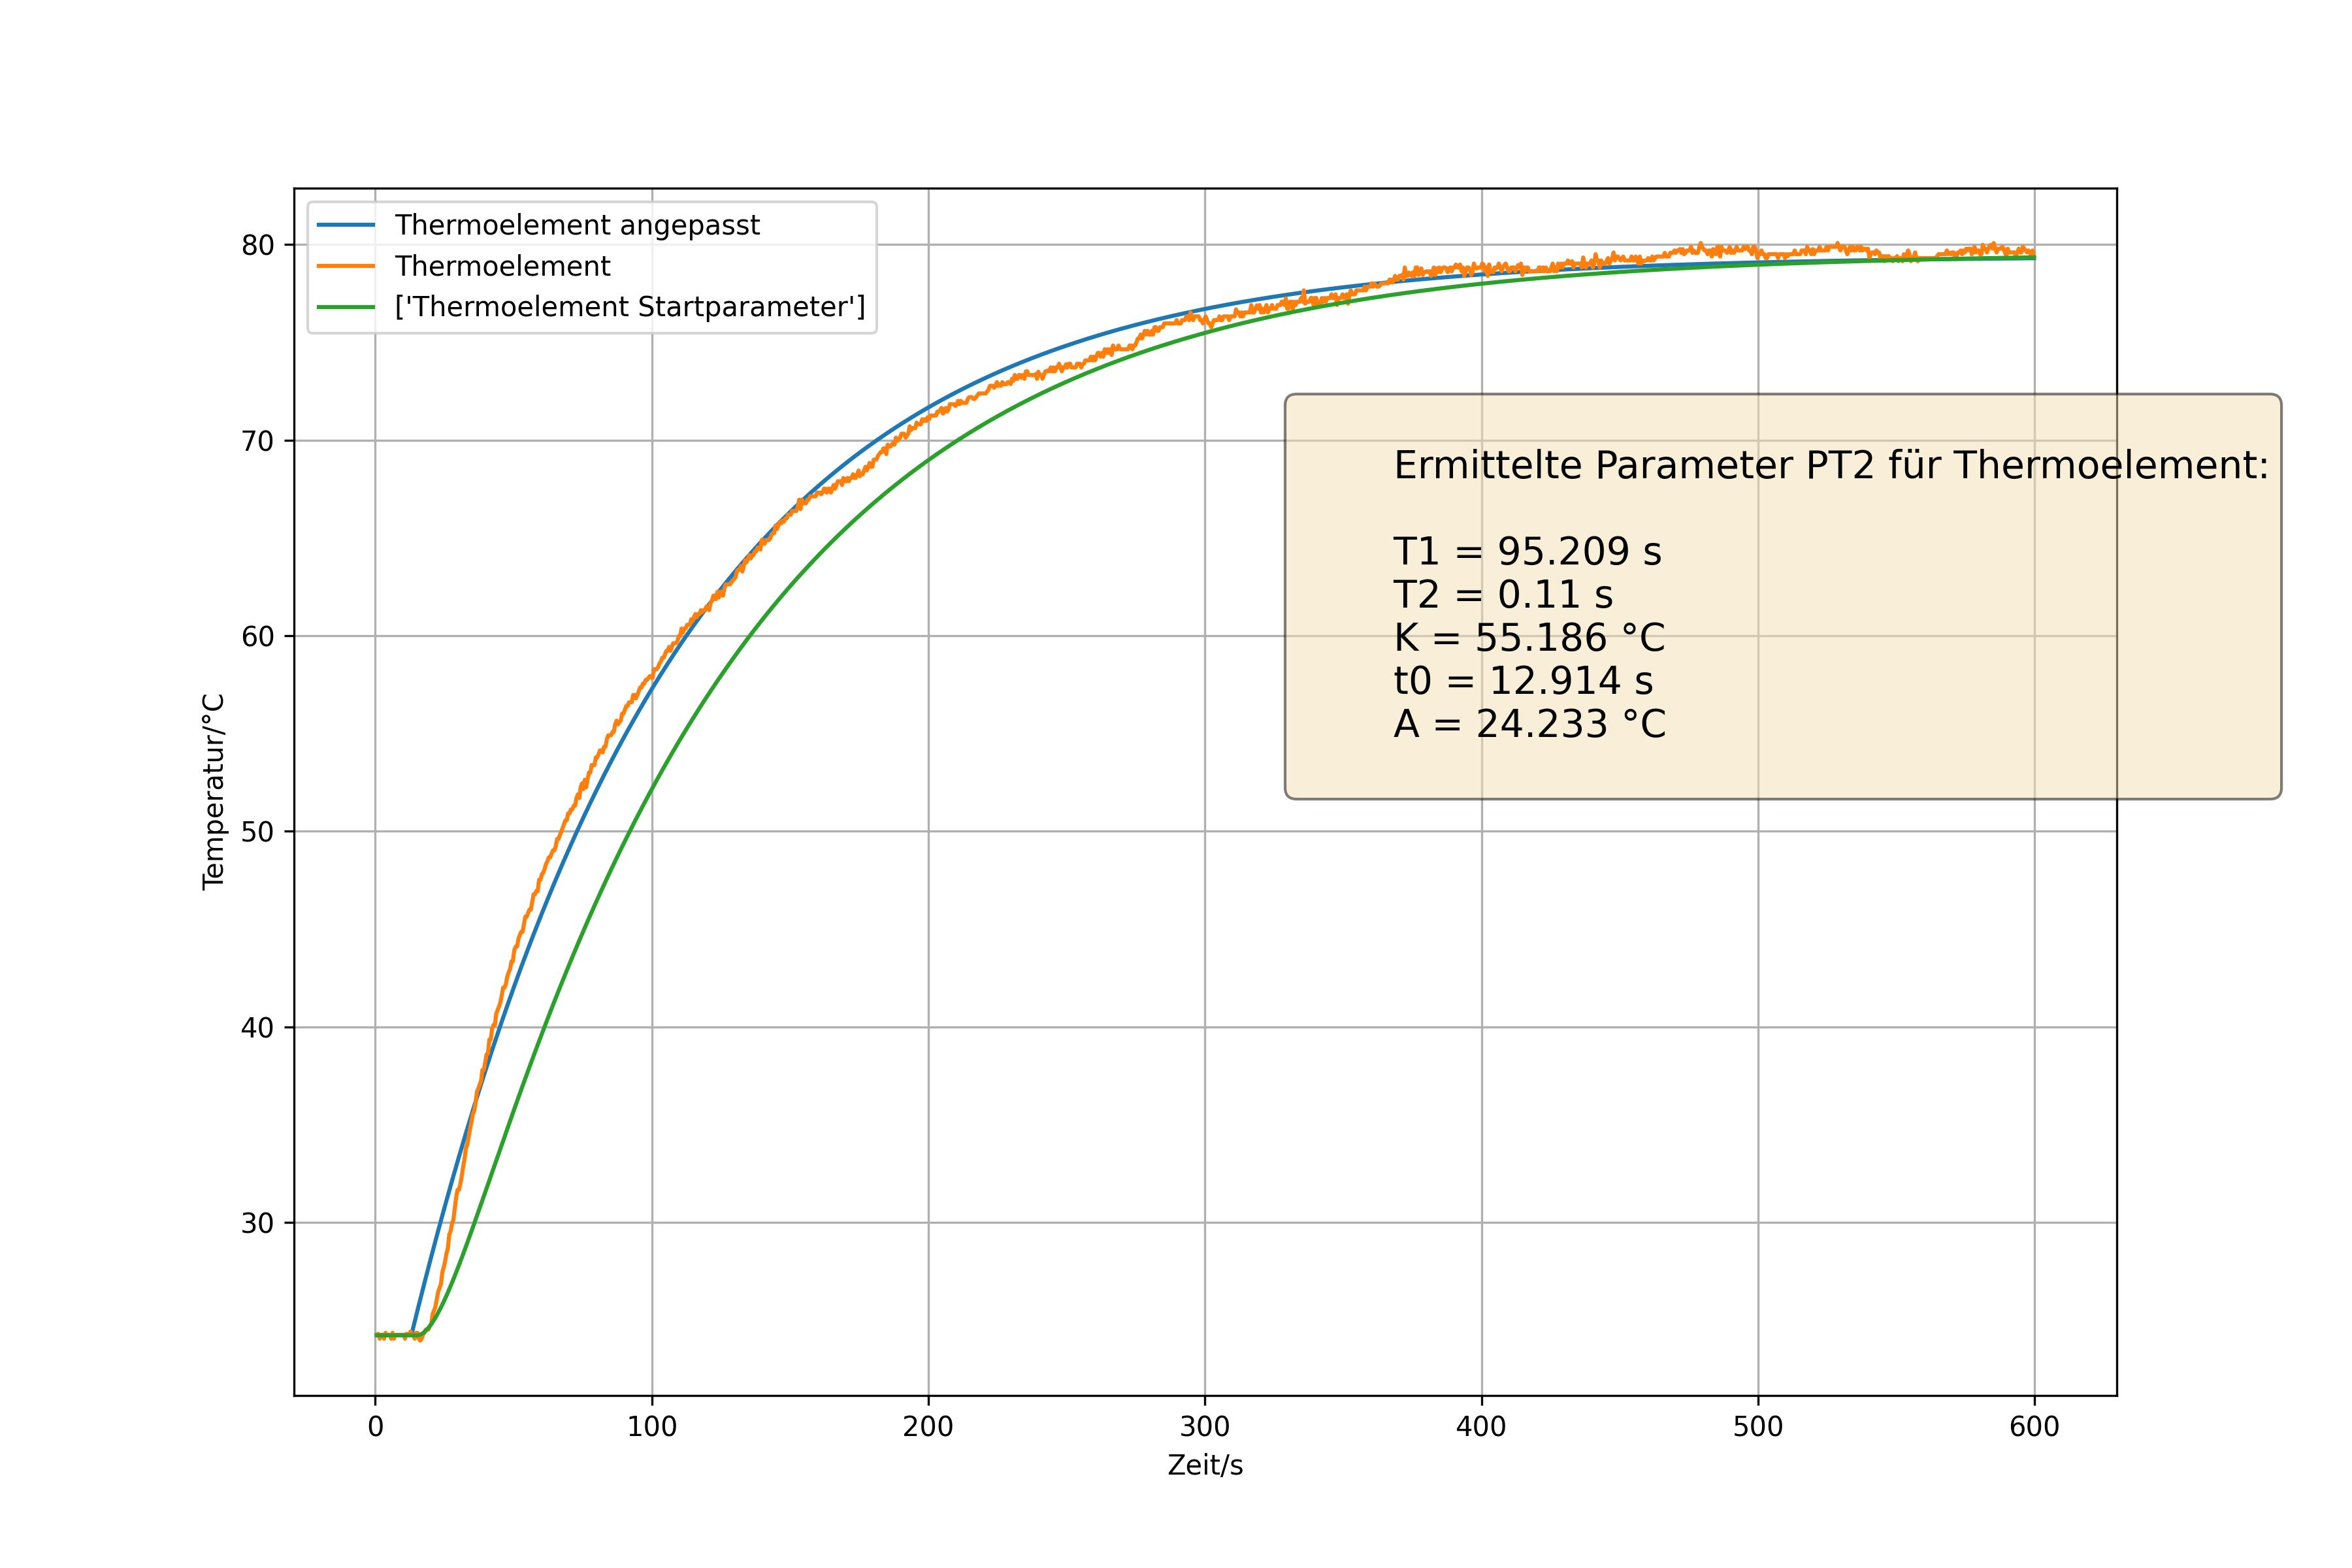
\includegraphics[width=0.9\textwidth]{data/auswertung/plotparameter_aufheiz_mit_scheibe16_19_00_TE_PT2.jpg}
    \caption{Plotparameter Aufheizphase mit Isolierung Thermoelement}
    \label{fig:plotparam_aufheiz_mit_isolierung_te}
\end{figure}
\begin{figure}[H]
    \centering
    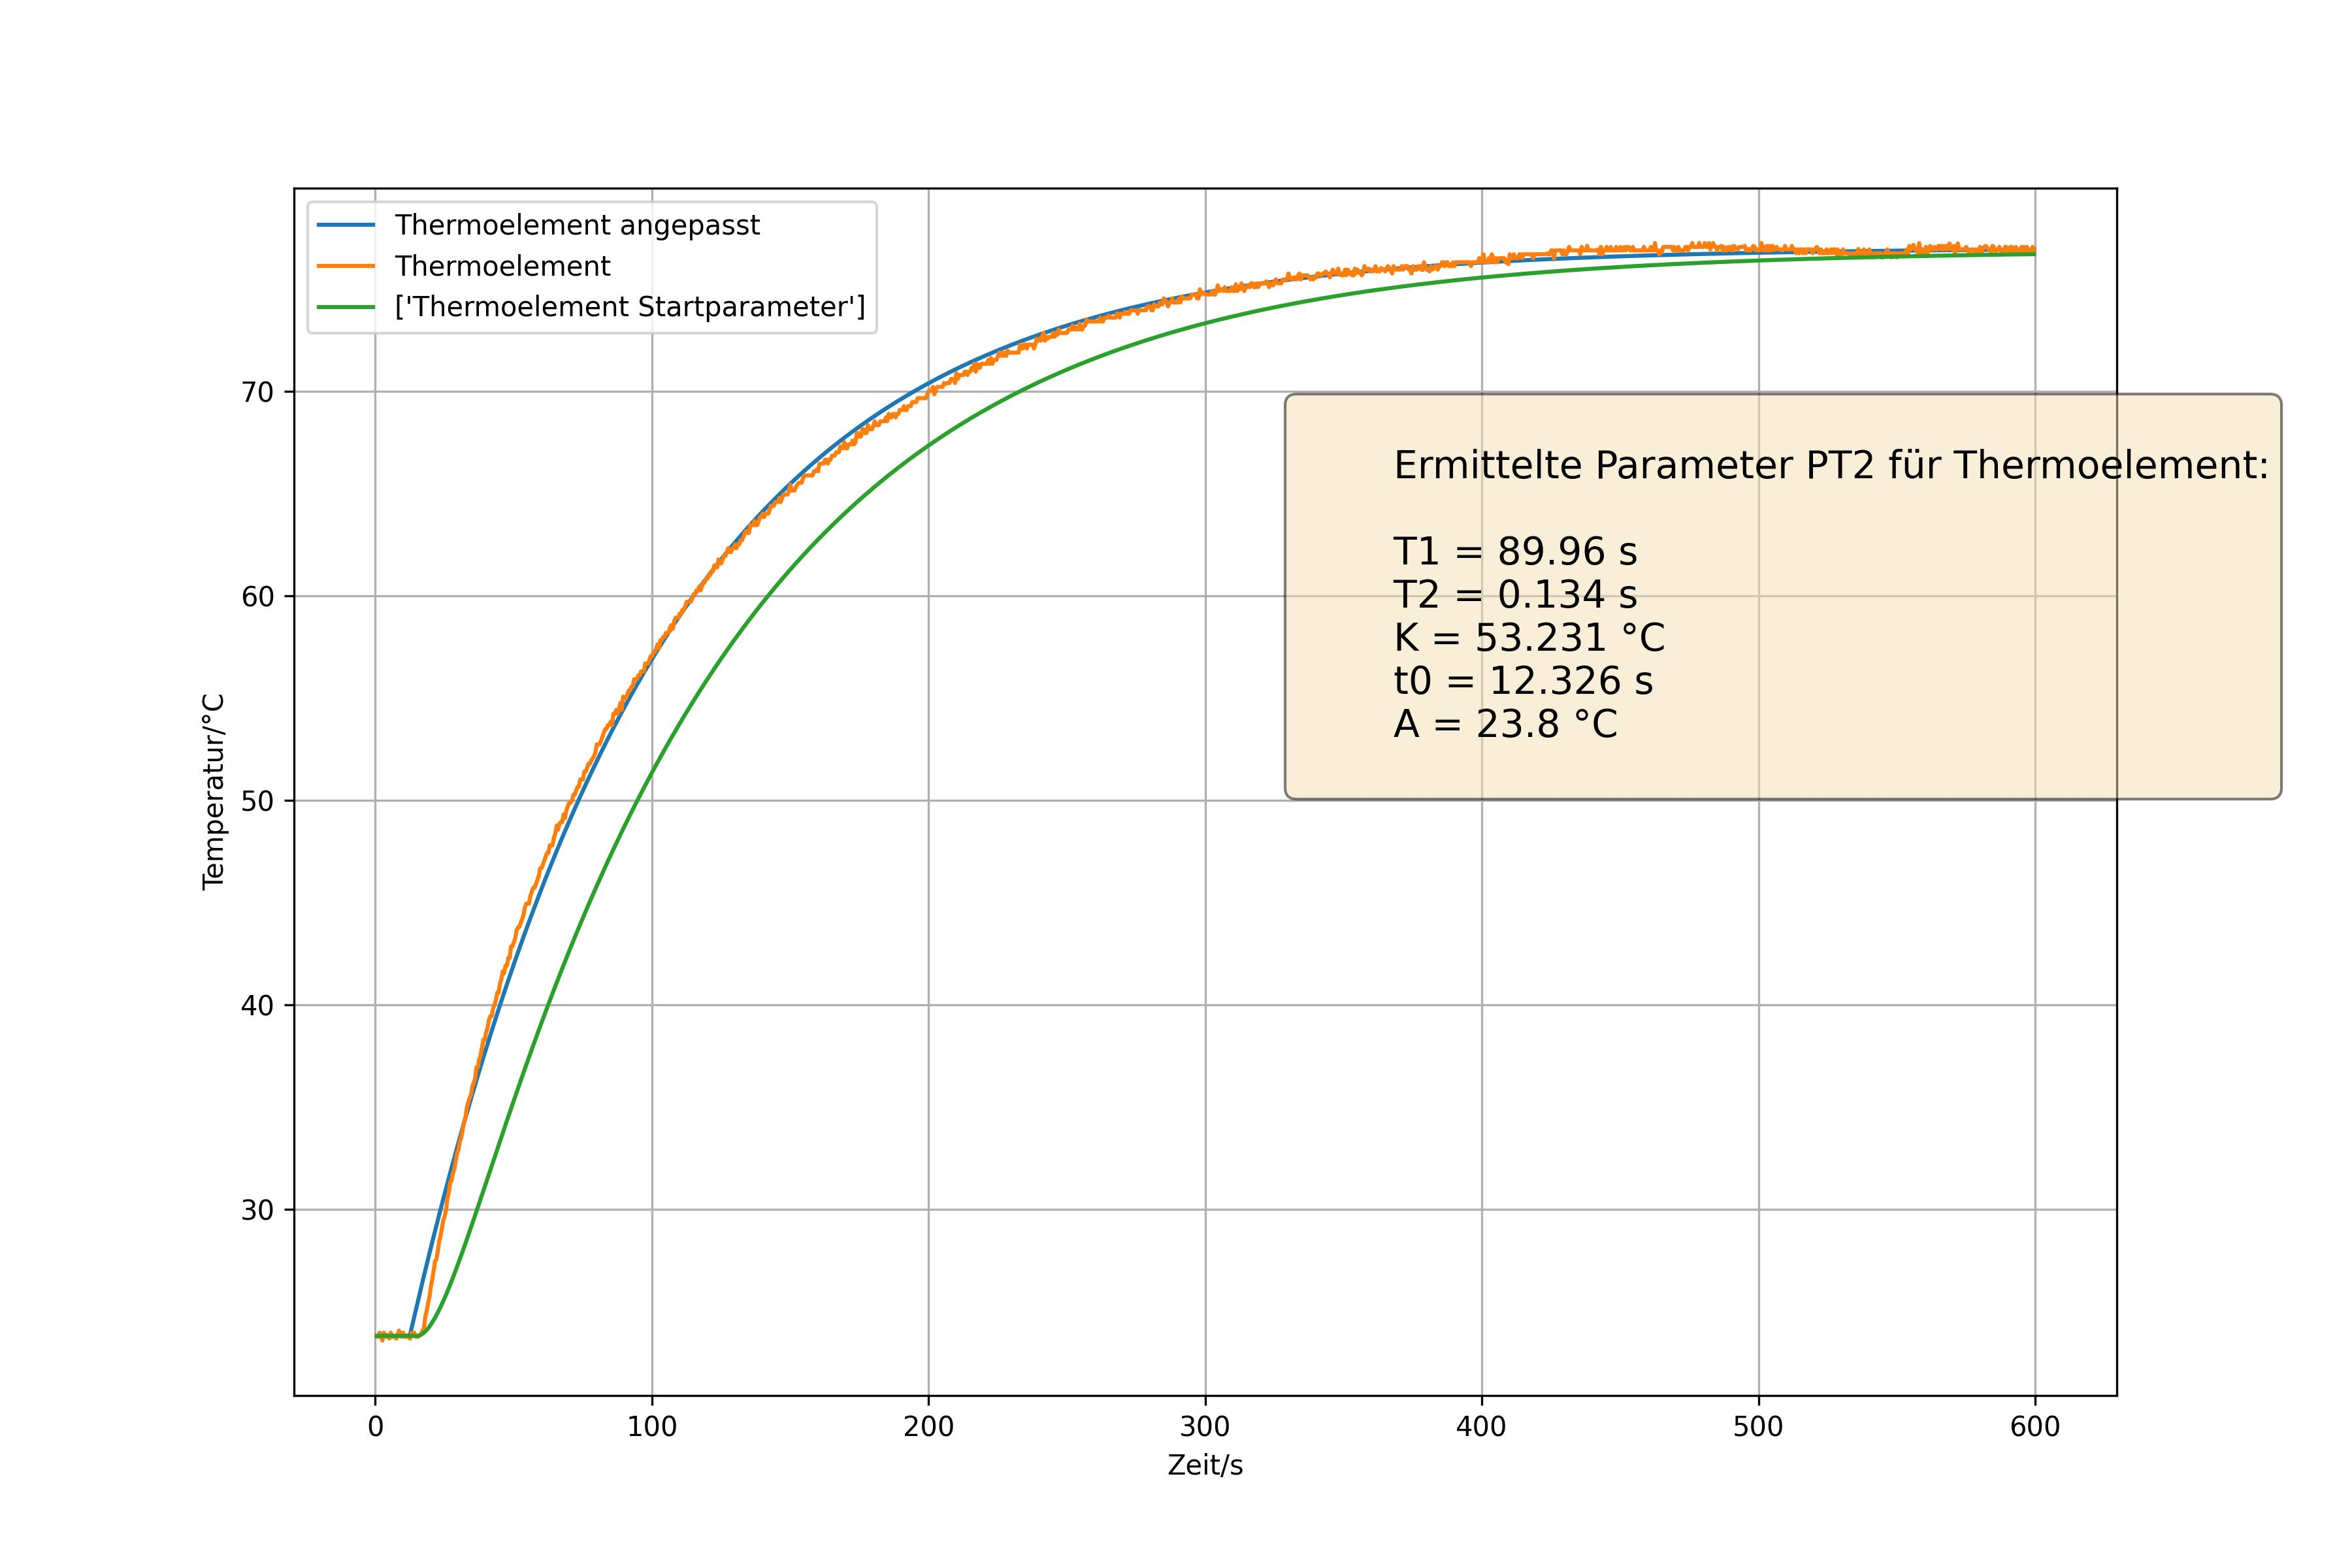
\includegraphics[width=0.9\textwidth]{data/auswertung/plotparameter_aufheiz_ohne_scheibe16_18_59_TE_PT2.jpg}
    \caption{Plotparameter Aufheizphase ohne Isolierung Thermoelement}
    \label{fig:plotparam_aufheiz_ohne_isolierung_te}
\end{figure}


\subsection{Abkühlphase}
Die Abkühlphase erstreckt sich in einem Zeitberich von ca. \SI{610}{\second} bis \SI{1220}{\second}. In diesem Zeitraum kühlen die Transistoren von ihrer Beharrungstemperatur wieder auf Raumtemperatur ab.
\begin{figure}[H]
    \centering
    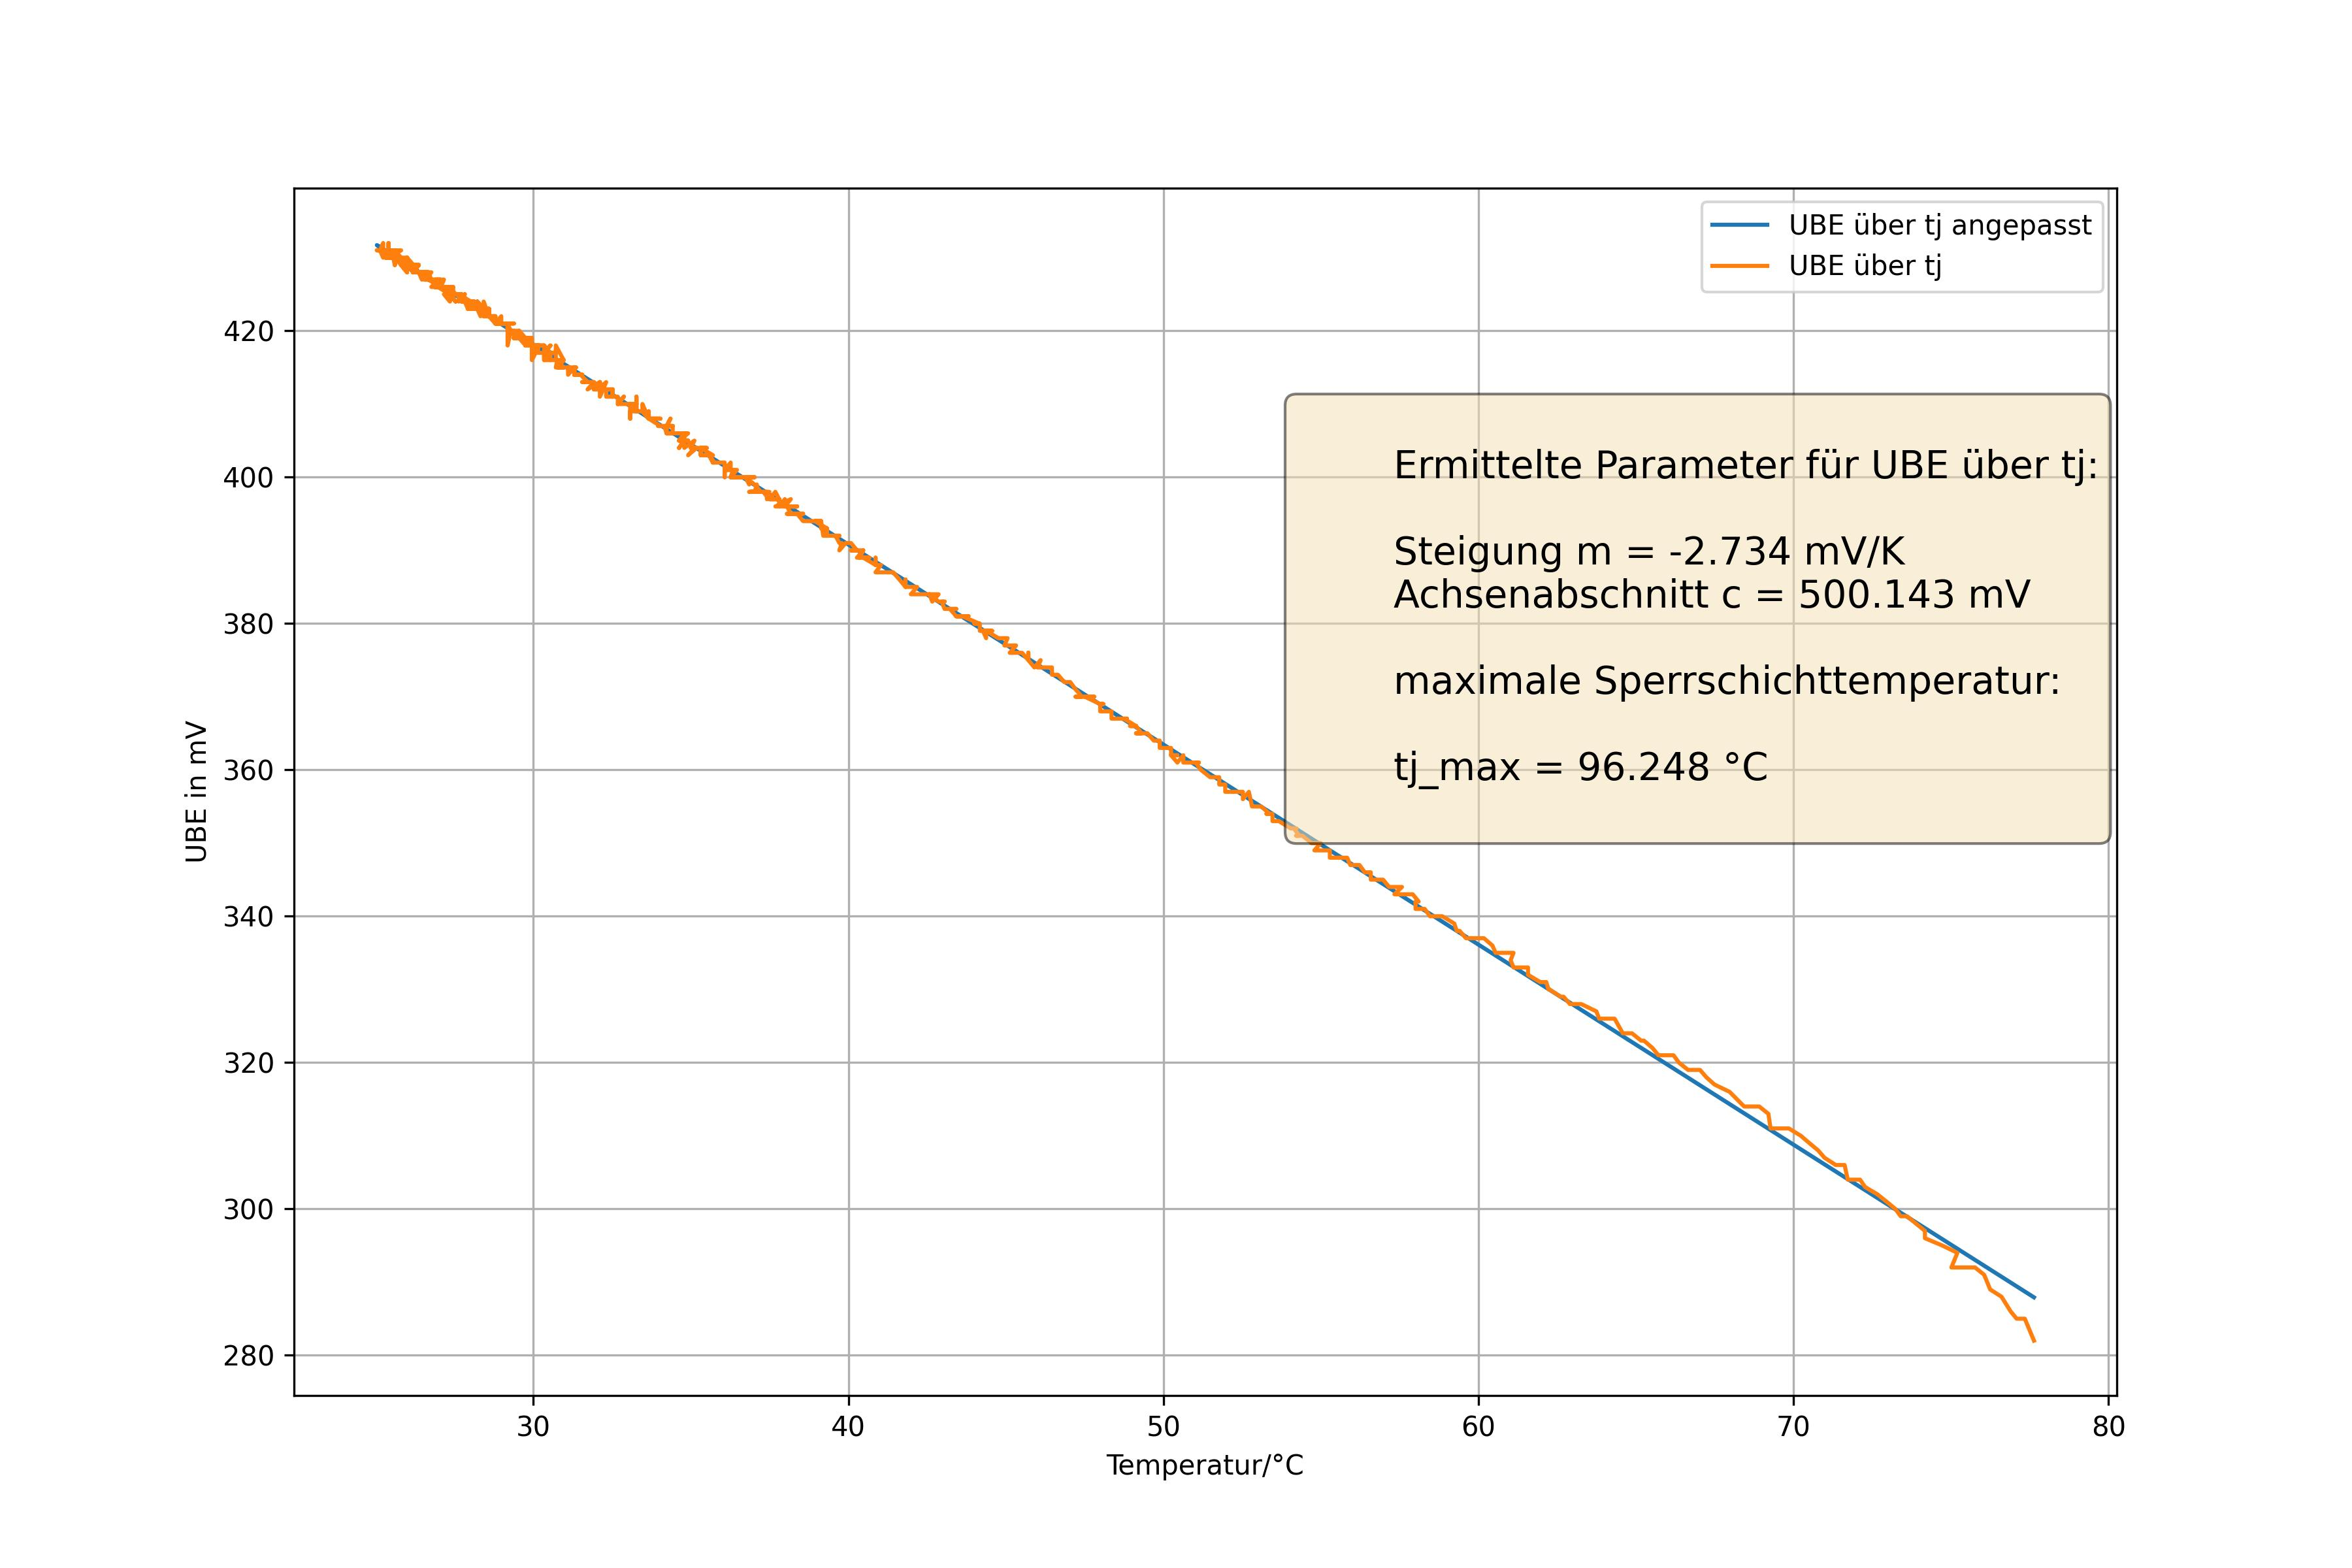
\includegraphics[width=0.9\textwidth]{data/auswertung/plotparameter_abkühl_mit_scheibe11_16_37_TE_Linear.jpg}
    \caption{Plotparameter Abkühlphase mit Isolierung Thermoelement}
    \label{fig:plotparam_abkuehl_mit_isolierung_te}
\end{figure}
\begin{figure}[H]
    \centering
    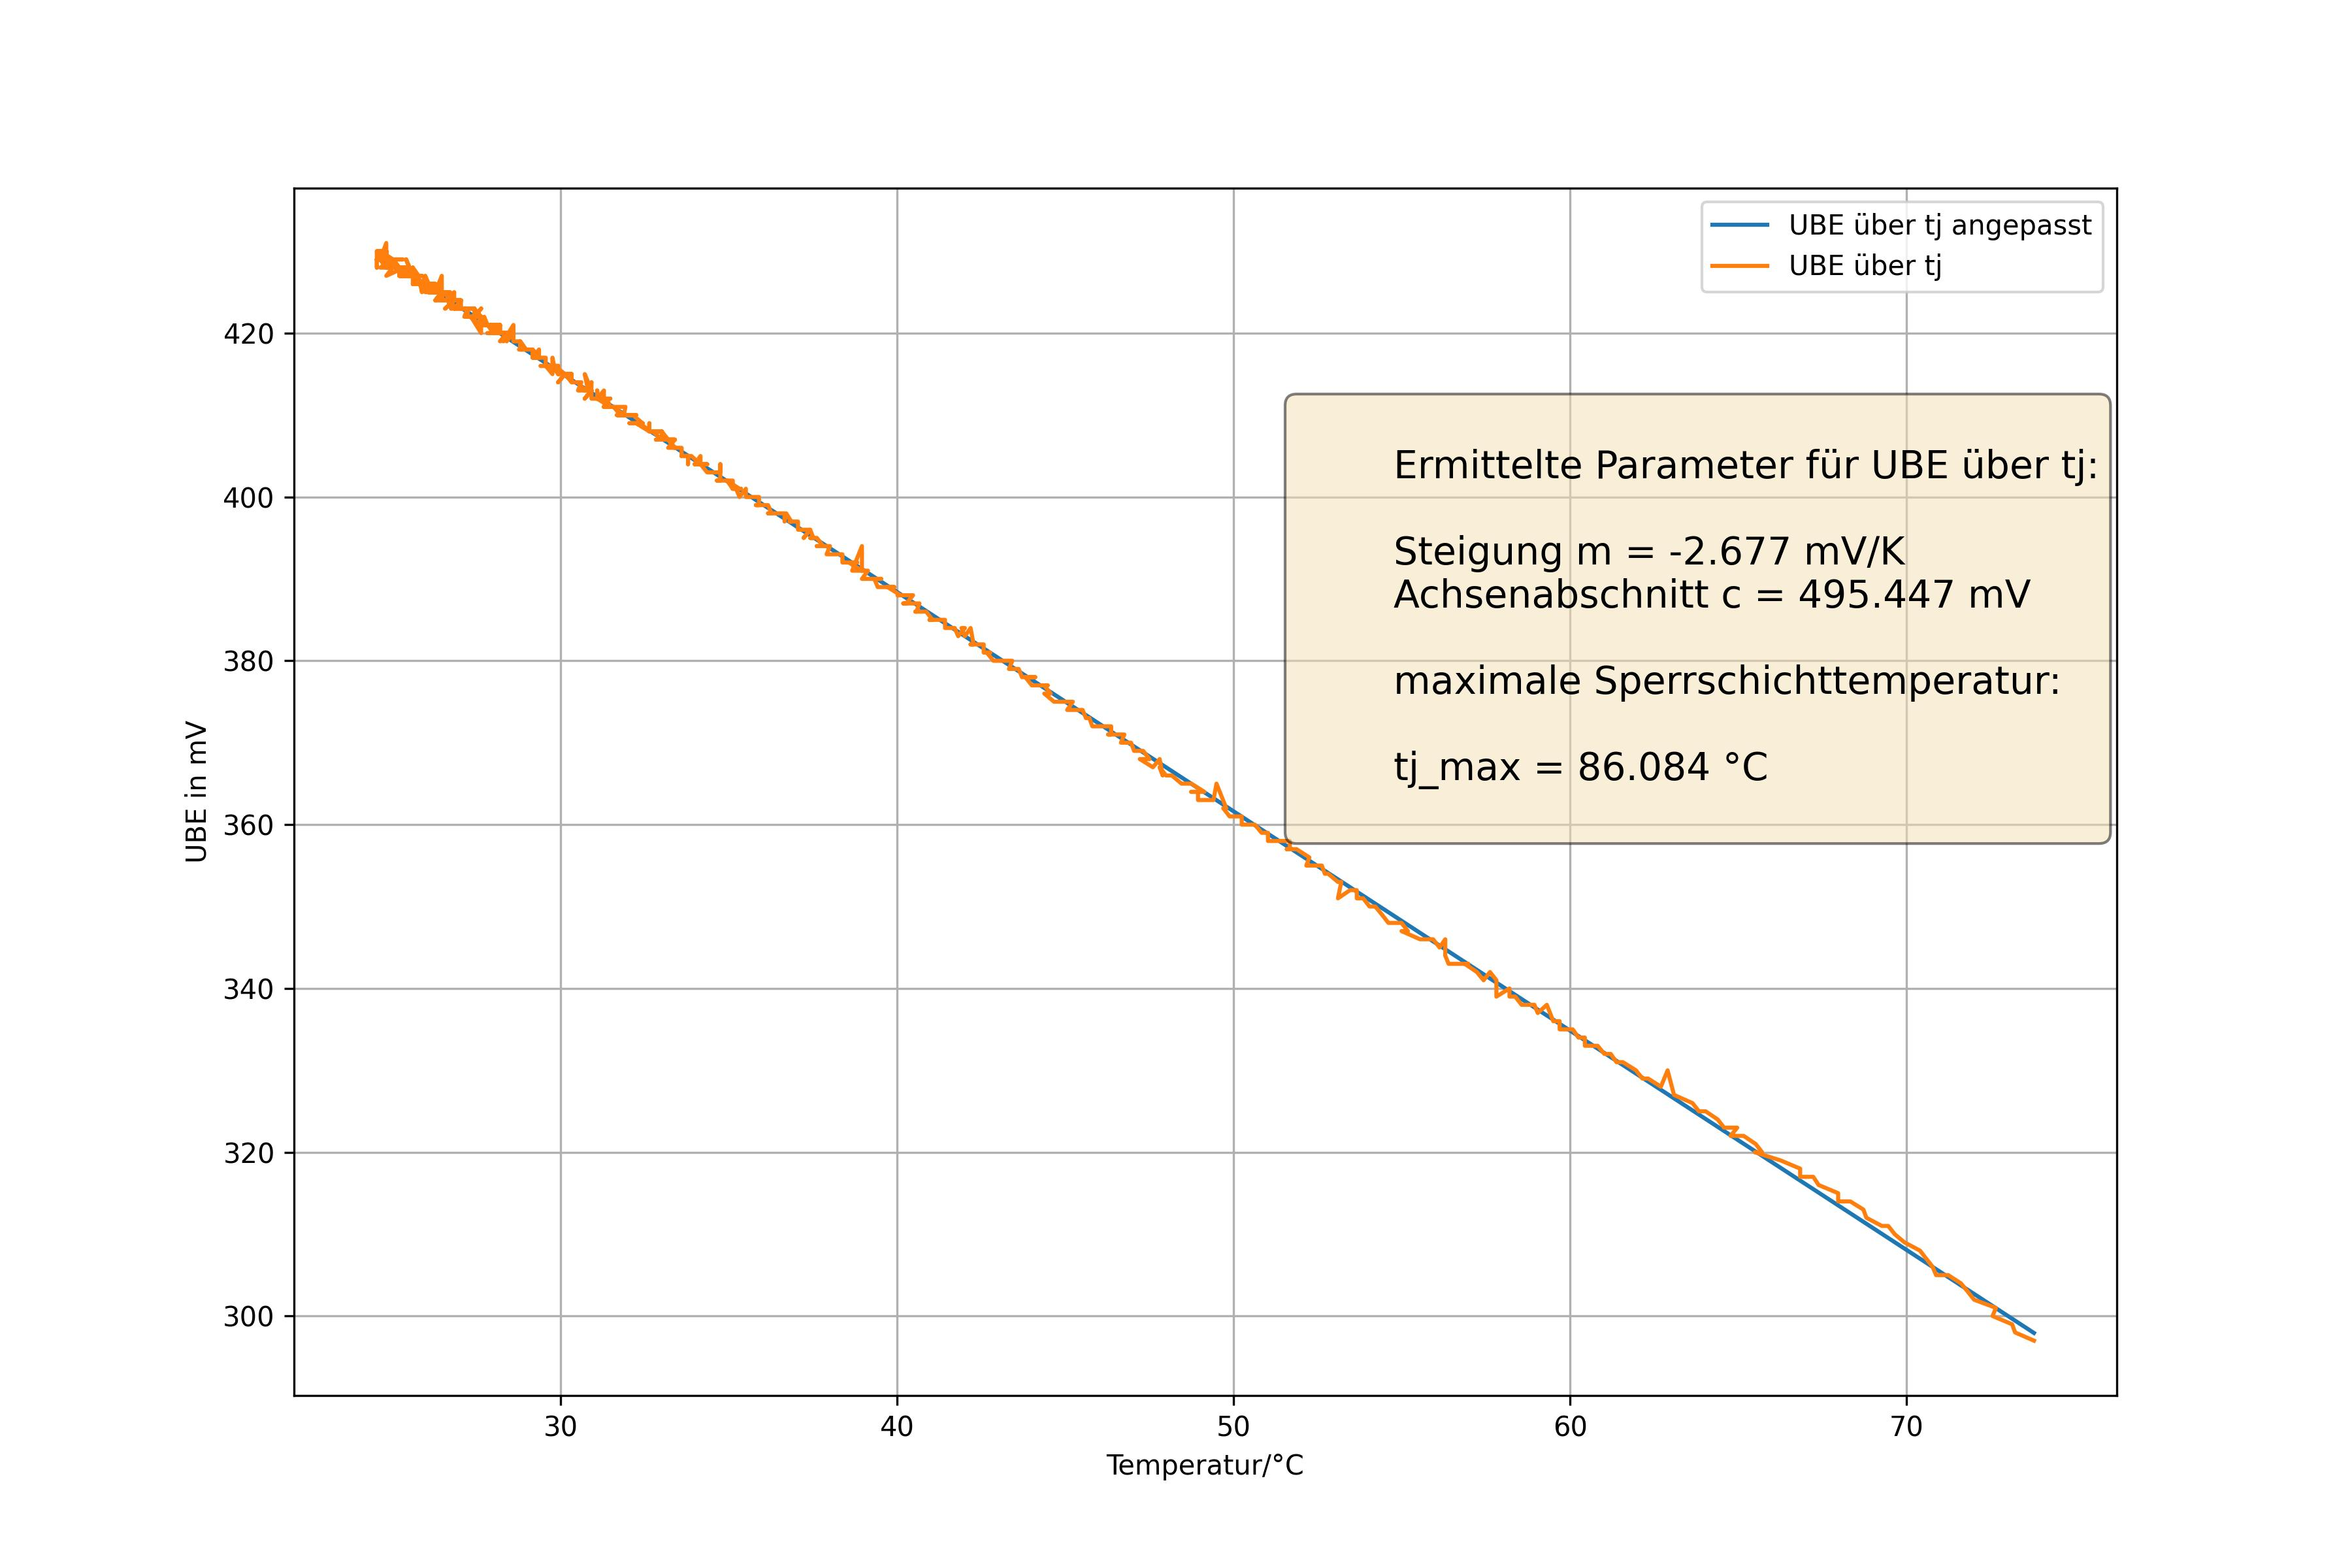
\includegraphics[width=0.9\textwidth]{data/auswertung/plotparameter_abkühl_ohne_scheibe11_16_36_TE_Linear.jpg}
    \caption{Plotparameter Abkühlphase ohne Isolierung Thermoelement}
    \label{fig:plotparam_abkuehl_ohne_isolierung_te}
\end{figure}

\subsection{Berechnung der Werte}

\subsubsection{Verlustleistung}
\label{scn:berechnung_verlustleistung}
Aus den Messdaten kann man die maximale $U_{CE}$ und $I_C$ Werte entnehmen:
\begin{equation}
    U_{CE} = \SI{2.93}{\volt}, \quad I_C = \SI{1.44}{\ampere}
\end{equation}
$U_{CE}$ und $I_C$ sind die maximalen Werte aus den Messdaten.
Damit ergibt sich die Verlustleistung zu:
\begin{equation}
    P_V = U_{CE} \cdot I_C = \SI{2.93}{\volt} \cdot \SI{1.44}{\ampere} = \boxed{\SI{4.2192}{\watt}}
\end{equation}

\subsubsection{Temperaturen}
\label{scn:anal_temp}
Die Kühlkörpertemperatur $\vartheta_S$ wird als Mittelwert der beiden NTC-Sensoren berechnet:
\begin{equation}
    \vartheta_S = \frac{\vartheta_{NTC1} + \vartheta_{NTC2}}{2}
\end{equation}
\begin{align*}
        \vartheta_S &= \frac{61.514 + 60.459}{2} \, \si{\degreeCelsius} = \boxed{\SI{60.9865}{\degreeCelsius}} \quad \text{(Mit Isolierung)} \\
        \vartheta_S &= \frac{62.528 + 61.539}{2} \, \si{\degreeCelsius} = \boxed{\SI{62.0335}{\degreeCelsius}} \quad \text{(Ohne Isolierung)}
\end{align*}
Die Gehäusetemperatur $\vartheta_C$ wird direkt aus dem Thermoelement abgelesen.
\begin{align*}
        \vartheta_C & = \boxed{\SI{79.586}{\degreeCelsius}} \quad \text{(Mit Isolierung)} \\
        \vartheta_C & = \boxed{\SI{76.913}{\degreeCelsius}} \quad \text{(Ohne Isolierung)}
\end{align*}
Um die maximale Sperrschichttemperatur $\vartheta_{J,max}$ zu bestimmen, wird die Temperaturabhängigkeit der Basis-Emitter-Spannung $U_{BE}$ genutzt. Da die Sperrschicht im Betrieb nicht direkt zugänglich ist, wird das Verhalten in der Abkühlphase analysiert. Nach dem Abschalten der Heizleistung gleichen sich die Sperrschichttemperatur $\vartheta_J$ und die Gehäusetemperatur $\vartheta_C$ schnell an, da kein Wärmestrom mehr von innen nach außen fließt. In diesem Zustand kann $\vartheta_C$ (gemessen mit dem Thermoelement) als Referenz für $\vartheta_J$ angenommen werden.

Mithilfe des Python-Programms wird eine lineare Regression durchgeführt, um die Kennlinie $U_{BE}(\vartheta) = m \cdot \vartheta + c$ zu bestimmen. Das Programm nutzt diese kalibrierte Kennlinie, um aus dem minimalen $U_{BE}$-Wert (gemessen unmittelbar beim Abschalten, als der Transistor am heißesten war) die maximale Sperrschichttemperatur $\vartheta_{J,max}$ zurückzurechnen.

Die ermittelten maximalen Sperrschichttemperaturen lauten:
\begin{align*}
    \vartheta_{J,max} &= \boxed{\SI{96.248}{\degreeCelsius}} \quad \text{(Mit Isolierung)} \\
    \vartheta_{J,max} &= \boxed{\SI{86.084}{\degreeCelsius}} \quad \text{(Ohne Isolierung)}
\end{align*}


\subsubsection{Wärmewirderstände}

Aus den ermittelten Beharrungstemperaturen und der elektrischen Verlustleistung $P_V$ lassen sich die Wärmewiderstände des Systems berechnen. Die Verlustleistung im stationären Zustand ergibt sich aus den Messdaten kurz vor dem Abschalten ($P_V = U_{CE} \cdot I_C$).

Die Wärmewiderstände berechnen sich analog zum Ohm'schen Gesetz aus der Temperaturdifferenz geteilt durch den Wärmestrom (Verlustleistung) :
\begin{align}
    R_{thJC} & = \frac{\vartheta_{J,max} - \vartheta_C}{P_V} \label{eq:RthJC} \\
    R_{thCS} & = \frac{\vartheta_C - \vartheta_S}{P_V} \label{eq:RthCS}       \\
    R_{thS}  & = \frac{\vartheta_S - \vartheta_U}{P_V} \label{eq:RthS}
\end{align}
Zur Ermittlung der Temperaturen siehe Abschnitt \ref{scn:anal_temp}.
\begin{align}
    R_{thJC} & = \frac{96.248 - 79.586}{4.2192} \, \si{\kelvin\per\watt} = \boxed{\SI{3.94}{\kelvin\per\watt}} \quad \text{(Mit Isolierung)} \\
    R_{thJC} & = \frac{86.084 - 76.913}{4.2192} \, \si{\kelvin\per\watt} = \boxed{\SI{2.18}{\kelvin\per\watt}} \quad \text{(Ohne Isolierung)} \\
    R_{thCS} & = \frac{79.586 - 60.9865}{4.2192} \, \si{\kelvin\per\watt} = \boxed{\SI{4.41}{\kelvin\per\watt}} \quad \text{(Mit Isolierung)} \\
    R_{thCS} & = \frac{76.913 - 62.0335}{4.2192} \, \si{\kelvin\per\watt} = \boxed{\SI{3.49}{\kelvin\per\watt}} \quad \text{(Ohne Isolierung)} \\
    R_{thS}  & = \frac{60.9865 - 22}{4.2192} \, \si{\kelvin\per\watt} = \boxed{\SI{9.26}{\kelvin\per\watt}} \quad \text{(Mit Isolierung)} \\
    R_{thS}  & = \frac{62.0335 - 22}{4.2192} \, \si{\kelvin\per\watt} = \boxed{\SI{9.52}{\kelvin\per\watt}} \quad \text{(Ohne Isolierung)}
\end{align}
\\
Tabelle \ref{tab:ergebnisse_gesamt} fasst die berechneten Parameter für beide Versuchsteile zusammen.

\subsection{Zusammenfassung der Ergebnisse}
\begin{table}[H]
    \centering
    \renewcommand{\arraystretch}{1.3}
    \begin{tabular}{l|c|c}
        \toprule
        \textbf{Parameter}                         & \textbf{Ohne Isolierscheibe}  & \textbf{Mit Isolierscheibe}   \\
        \midrule
        Verlustleistung $P_V$                      & \SI{4.2192}{\watt}            & \SI{4.2192}{\watt}            \\
        Kühlkörpertemp. $\vartheta_S$ (Mittelwert) & \SI{62.0335}{\degreeCelsius}  & \SI{60.9865}{\degreeCelsius}  \\
        Gehäusetemperatur $\vartheta_C$            & \SI{76.913}{\degreeCelsius}   & \SI{79.586}{\degreeCelsius}   \\
        Sperrschichttemperatur $\vartheta_{J,max}$ & \SI{86.084}{\degreeCelsius}   & \SI{96.248}{\degreeCelsius}   \\
        \midrule
        $R_{thJC}$ (Sperrschicht - Gehäuse)        & \SI{2.18}{\kelvin\per\watt}   & \SI{3.94}{\kelvin\per\watt}   \\
        $R_{thCS}$ (Gehäuse - Kühlkörper)          & \SI{3.49}{\kelvin\per\watt}   & \SI{4.41}{\kelvin\per\watt}   \\
        $R_{thS}$ (Kühlkörper - Umgebung)          & \SI{9.52}{\kelvin\per\watt}   & \SI{9.26}{\kelvin\per\watt}   \\
        \midrule
        Zeitkonstante $\tau$                       & \SI{89.960}{\second}          & \SI{95.209}{\second}          \\
        \bottomrule
    \end{tabular}
    \caption{Tabellarische Übersicht der messtechnisch ermittelten Parameter}
    \label{tab:ergebnisse_gesamt}
\end{table}
Die gemessenen Werte für die Wärmewiderstände weichen von den im Vorbereitungsteil berechneten Werten ab. Dies kann auf Messungenauigkeiten, Abweichungen in den Materialeigenschaften und vereinfachte Annahmen im theoretischen Modell zurückgeführt werden. Der Fehler wird in Kapitel \ref{scn:fehler_waermewiderstand} näher erläutert.
\section{Fehlerbetrachtung von Wärmewiderständen}
\label{scn:fehler_waermewiderstand}
In Tabelle \ref{tab:vergleich_rth} werden die in der Vorbereitung berechneten Wärmewiderstände mit den experimentell ermittelten Werten verglichen.

\begin{table}[H]
    \centering
    \renewcommand{\arraystretch}{1.3}
    \begin{tabular}{l|c|c|c}
        \toprule
        \textbf{Wärmewiderstand}                  & \textbf{Vorbereitung} & \textbf{Messung (ohne Iso.)} & \textbf{Messung (mit Iso.)} \\
        \midrule
        $R_{th,JC}/{\si{\kelvin\per\watt}}$       & \num{3.13}            & \num{2.18}                   & \num{3.94}                  \\
        $R_{th,CS}/{\si{\kelvin\per\watt}}$       & \num{1.00}            & \num{3.49}                   & --                          \\
        $R_{th,CS, iso}/{\si{\kelvin\per\watt}}$  & \num{2.00}            & --                           & \num{4.41}                  \\
        $R_{th,S}/{\si{\kelvin\per\watt}}$        & \num{15.00}           & \num{9.52}                   & \num{9.26}                  \\
        \midrule
        $R_{th,ges}/{\si{\kelvin\per\watt}}$      & \num{19.13}           & \num{15.19}                  & --                          \\
        $R_{th,ges, iso}/{\si{\kelvin\per\watt}}$ & \num{20.13}           & --                           & \num{17.61}                 \\
        \bottomrule
    \end{tabular}
    \caption{Vergleich der Wärmewiderstände: Vorbereitung vs. Messung}
    \label{tab:vergleich_rth}
\end{table}

Die prozentuale Abweichung zwischen den theoretisch berechneten und den experimentell ermittelten Werten ist in Tabelle \ref{tab:abweichung_rth} dargestellt.

\begin{table}[H]
    \centering
    \renewcommand{\arraystretch}{1.3}
    \begin{tabular}{l|c|c}
        \toprule
        \textbf{Wärmewiderstand} & \textbf{Abweichung (ohne Iso.)} & \textbf{Abweichung (mit Iso.)} \\
        \midrule
        $R_{th,JC}$              & \SI{-30.35}{\percent}           & \SI{+25.88}{\percent}          \\
        \midrule
        $R_{th,CS}$              & \SI{+249.00}{\percent}          & --                             \\
        $R_{th,CS, iso}$         & --                              & \SI{+120.50}{\percent}         \\
        \midrule
        $R_{th,S}$               & \SI{-36.53}{\percent}           & \SI{-38.27}{\percent}          \\
        \midrule
        $R_{th,ges}$             & \SI{-20.60}{\percent}           & --                             \\
        $R_{th,ges, iso}$        & --                              & \SI{-12.52}{\percent}          \\
        \bottomrule
    \end{tabular}
    \caption{Prozentuale Abweichung der Wärmewiderstände (Messung vs. Vorbereitung)}
    \label{tab:abweichung_rth}
\end{table}

Man erkennt hier, dass bei der Messung des Wärmewiderstands eine deutliche Abweichung zu den in der Vorbereitung berechneten Werten besteht, insbesondere für den Wärmewiderstand $R_{th,CS}$. Grund hierfür können verschiedene Faktoren sein. Der Kühlkörper war mit einer Schraube befestigt, die den Wärmeübergang beeinflussen kann. Wenn die Schraube nicht fest genug angezogen ist, kann dies den Wärmeübergang drastisch verschlechtern. Dies würde die hohe Abweichung erklären. Zudem können Messfehler bei der Temperatur- und Spannungsmessung sowie Abweichungen in den Materialeigenschaften der Bauteile zu Ungenauigkeiten führen.


\subsection{Fehlerfortpflanzung}
Allgemein lassen sich die Wärmewiderstände wie folgt berechnen:
\begin{equation*}
    R_{thJC} = f(\vartheta_J, \vartheta_C, I_C, U_{CE}) = \frac{\Delta \vartheta_{JC}}{P_V} = \frac{\vartheta_J - \vartheta_C}{I_C \cdot U_{CE}}
\end{equation*}
Die Wärmewiderstände hängen von der Temperaturdifferenz $\Delta \vartheta$ und der Verlustleistung $P_V$ ab. Beide Messgrößen leiden unter systematische Messfehler und Messunsicherheiten aufgrund von nicht-idealen Messgeräten und Bauteilen sowie menschlichen Fehlern.
Man nimmt hierfür einen Messsfehler von $\Delta \vartheta = \pm \SI{0.5}{\kelvin}$ an und jeweils eine Abweichung von $\pm 0.5\%$ für die Strom- und Spannungsmessung. Dies entspricht:
\begin{align*}
    \Delta I_C    & = \SI{0.5}{\percent} \cdot \SI{1.44}{\ampere} = \SI{0.0072}{\ampere} = \SI{7.2}{\milli\ampere} \\
    \Delta U_{CE} & = \SI{0.5}{\percent} \cdot \SI{2.93}{\volt} = \SI{0.01465}{\volt} = \SI{14.65}{\milli\volt}
\end{align*}
Da der Wärmewiderstand von der Verlustleistung $P_V$ und der Temperaturdifferenz $\Delta \vartheta$ abhängt, pflanzt sich der Fehler wie folgt fort:
\begin{align}
    \label{eqn:raw_fehlerfortpflanzung}
    \Delta R_{thJC} & = \left| \frac{\partial R_{thJC}}{\partial \vartheta_J} \right| \Delta \vartheta_J + \left| \frac{\partial R_{thJC}}{\partial \vartheta_C} \right| \Delta \vartheta_C + \left| \frac{\partial R_{thJC}}{\partial I_C} \right| \Delta I_C + \left| \frac{\partial R_{thJC}}{\partial U_{CE}} \right| \Delta U_{CE}  \\
                    & = \left| \frac{1}{I_C \cdot U_{CE}} \right| \Delta \vartheta_J + \left| \frac{1}{I_C \cdot U_{CE}} \right| \Delta \vartheta_C  + \left| \frac{\vartheta_J - \vartheta_C}{(I_C)^2 \cdot U_{CE}} \right| \Delta I_C  + \left| \frac{\vartheta_J - \vartheta_C}{I_C \cdot (U_{CE})^2} \right| \Delta U_{CE} \nonumber
\end{align}
Da $\Delta \vartheta_J = \Delta \vartheta_C = \Delta \vartheta$ gilt, kann man die obige Gleichung vereinfachen:
\begin{align}
    \Delta R_{thJC} & = 2 \cdot \left| \frac{1}{P_V} \right| \Delta \vartheta + \left| \frac{\Delta \vartheta_{JC}}{(I_C)^2 \cdot U_{CE}} \right| \Delta I_C + \left| \frac{\Delta \vartheta_{JC}}{I_C \cdot (U_{CE})^2} \right| \Delta U_{CE}
\end{align}
Mit den gemessenen Werten aus Kapitel \ref{scn:berechnung_verlustleistung} und den angenommenen Messfehlern ergibt sich somit für den Versuch ohne Isolierung ein Fehler von:
\begin{align*}
    \Delta R_{thJC} & = 2 \cdot \left| \frac{1}{\SI{4.2192}{\watt}} \right| \SI{0.5}{\kelvin} + \left| \frac{\SI{9.171}{\kelvin}}{(\SI{1.44}{\ampere})^2 \cdot \SI{2.93}{\volt}} \right| \SI{7.2}{\milli\ampere} + \left| \frac{\SI{9.171}{\kelvin}}{\SI{1.44}{\ampere} \cdot (\SI{2.93}{\volt})^2} \right| \SI{14.65}{\milli\volt} \\
                    & = \boxed{\SI{0.259}{\kelvin\per\watt}}
\end{align*}
\begin{align*}
     & \Rightarrow \Delta R_{thJC} \approx \pm \SI{0.26}{\kelvin\per\watt} \\
     & \Rightarrow \frac{\Delta R_{thJC}}{R_{thJC}} \approx \pm 11.93\%          %\approx \SI{0.26}{\kelvin\per\watt}
\end{align*}
Mit dem gleichen Vorgehen ergibt sich für den Versuch mit Isolierung ein Fehler von:
\begin{align*}
    \Delta R_{thJC, iso} & = 2 \cdot \left| \frac{1}{\SI{4.2192}{\watt}} \right| \SI{0.5}{\kelvin} + \left| \frac{\SI{16.662}{\kelvin}}{(\SI{1.44}{\ampere})^2 \cdot \SI{2.93}{\volt}} \right| \SI{7.2}{\milli\ampere} + \left| \frac{\SI{16.662}{\kelvin}}{\SI{1.44}{\ampere} \cdot (\SI{2.93}{\volt})^2} \right| \SI{14.65}{\milli\volt} \\
                         & = \boxed{\SI{0.277}{\kelvin\per\watt}}
\end{align*}\begin{align*}
     & \Rightarrow \Delta R_{thJC, iso} \approx \pm \SI{0.28}{\kelvin\per\watt} \\
     & \Rightarrow \frac{\Delta R_{thJC, iso}}{R_{thJC, iso}} \approx \pm 7.11\%      %\approx \SI{0.28}{\kelvin\per\watt}
\end{align*}
\section{Fazit}
Zusammenfassend kann gesagt werden, dass der Versuch erfolgreich die Auswirkungen unterschiedlicher Montagearten auf die Wärmeableitung eines Leistungshalbleiters demonstriert hat. Die Messungen zeigten deutlich, dass der Einsatz einer Isolierscheibe den Wärmewiderstand zwischen Gehäuse und Kühlkörper signifikant erhöht, was zu höheren Sperrschichttemperaturen und längeren Zeitkonstanten führt. 
Die experimentell ermittelten Wärmewiderstände wichen jedoch teilweise sehr stark von den theoretisch berechneten Werten ab, was auf verschiedene Fehlerquellen zurückgeführt werden kann, wie z.B. unzureichende Befestigung des Kühlkörpers oder Messungenauigkeiten.

\end{document}